% Cover 2: "Minimal Modernist" — White ground, bold cobalt geometric sigma, clean academic
\documentclass[tikz,border=0mm]{standalone}
\usepackage{tikz}
\usetikzlibrary{calc,shapes.geometric}
\usepackage{xcolor}
\usepackage[T1]{fontenc}

\definecolor{cream}{RGB}{252,250,245}
\definecolor{cobalt}{RGB}{0,71,171}
\definecolor{cobaltlight}{RGB}{60,120,210}
\definecolor{cobaltvlight}{RGB}{180,205,240}
\definecolor{darktext}{RGB}{20,25,40}
\definecolor{midtext}{RGB}{80,90,110}
\definecolor{accentred}{RGB}{190,30,45}

\begin{document}
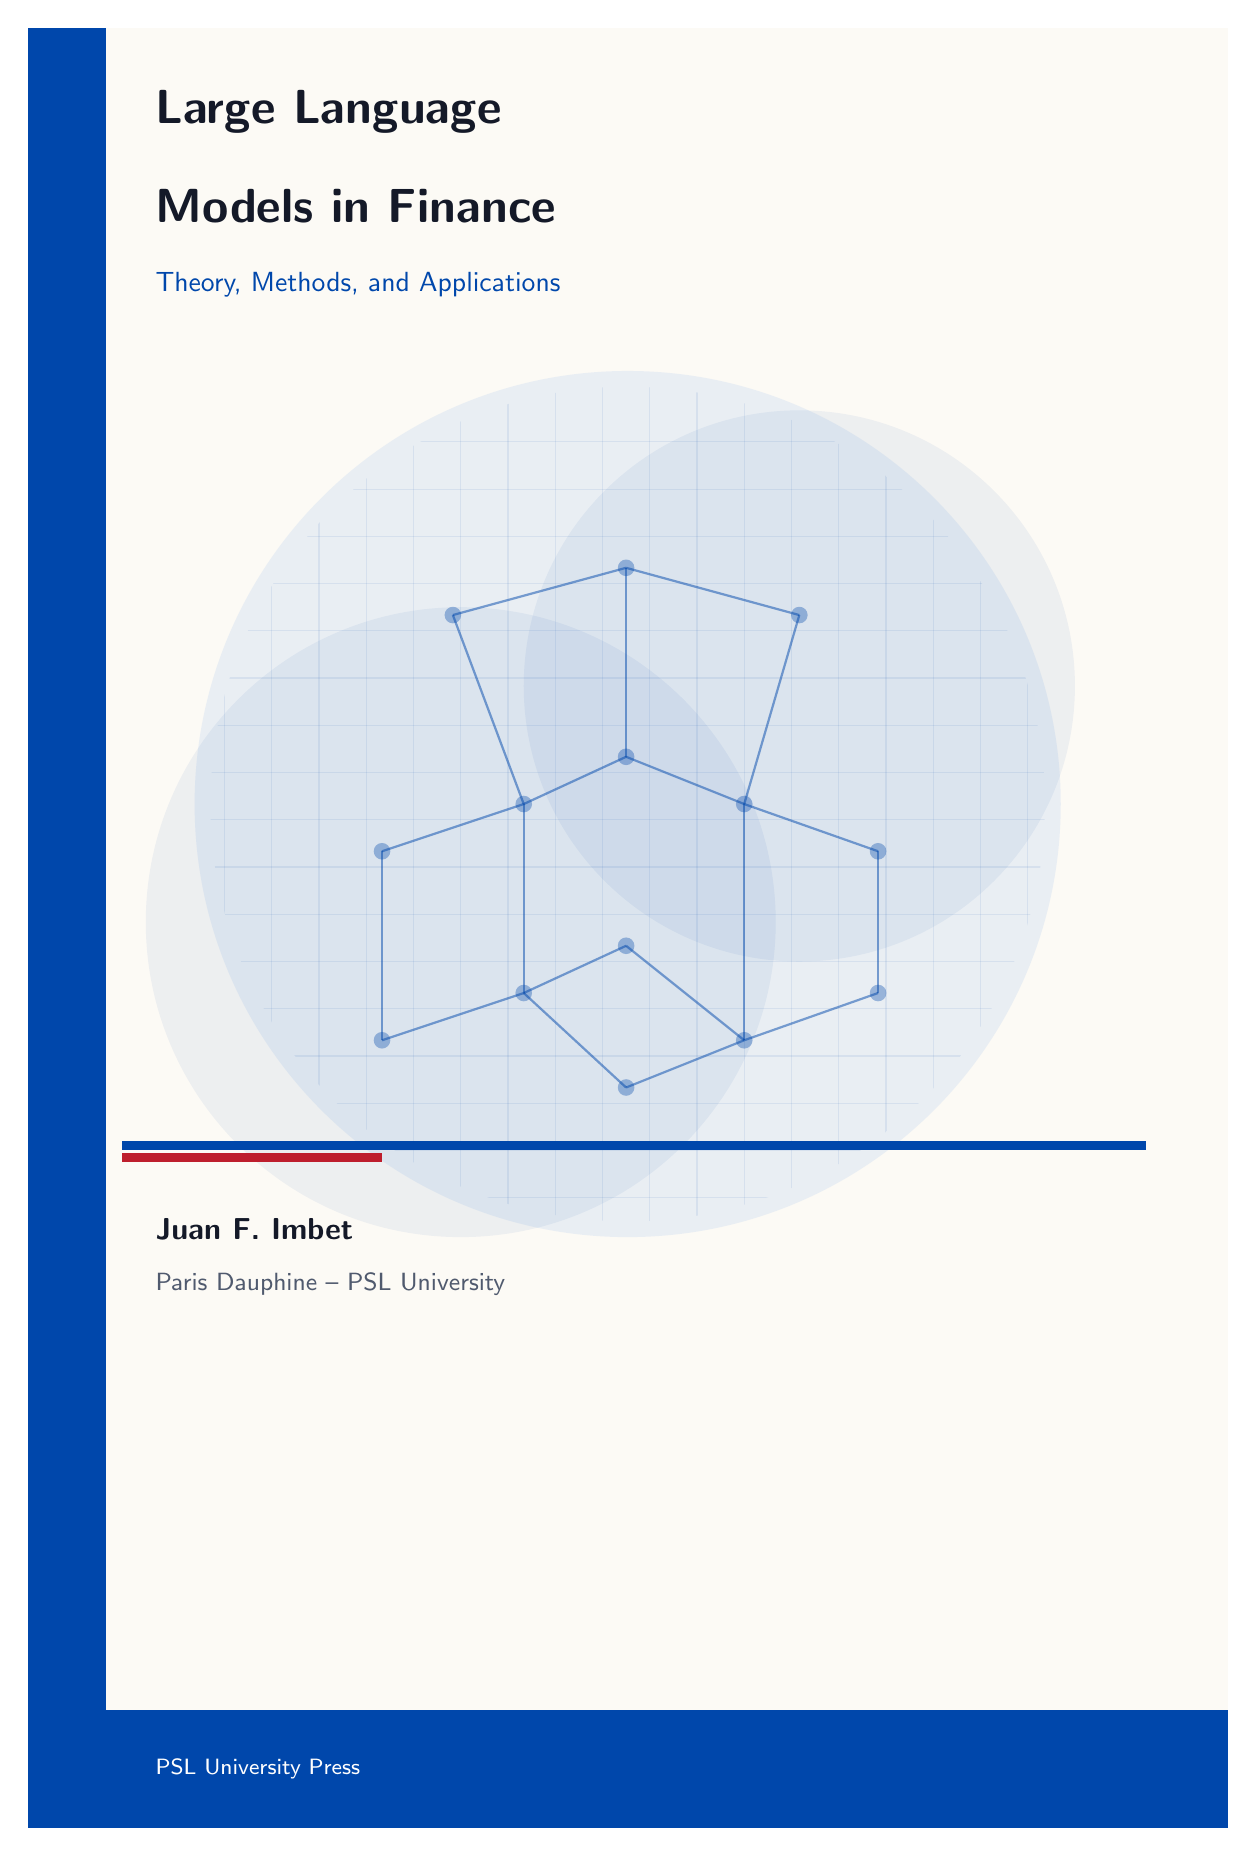
\begin{tikzpicture}
  % --- background ---
  \fill[cream] (0,0) rectangle (15.24,22.86);

  % --- bold left stripe ---
  \fill[cobalt] (0,0) rectangle (1.0,22.86);

  % --- large background geometric shape (Sigma / network icon) ---
  % Abstract large "brain network" shape: overlapping circles in very light blue
  \fill[cobaltvlight,opacity=0.25] (7.62,13.0) circle (5.5cm);
  \fill[cobalt,opacity=0.06] (5.5,11.5) circle (4.0cm);
  \fill[cobalt,opacity=0.06] (9.8,14.5) circle (3.5cm);

  % --- decorative circuit-like lines inside the circle area ---
  \begin{scope}
    \clip (7.62,13.0) circle (5.3cm);
    % horizontal lines
    \foreach \y in {8.0,8.6,...,18.0}{
      \draw[cobalt,opacity=0.08,line width=0.4pt] (2.0,\y) -- (13.5,\y);
    }
    % vertical lines
    \foreach \x in {2.5,3.1,...,13.5}{
      \draw[cobalt,opacity=0.08,line width=0.4pt] (\x,7.5) -- (\x,18.5);
    }
    % node dots at intersections (selective)
    \foreach \x/\y in {
      4.5/10.0, 6.3/10.6, 7.6/9.4, 9.1/10.0, 10.8/10.6,
      4.5/12.4, 6.3/13.0, 7.6/13.6, 9.1/13.0, 10.8/12.4,
      5.4/15.4, 7.6/16.0, 9.8/15.4, 7.6/11.2
    }{
      \fill[cobalt,opacity=0.35] (\x,\y) circle (3pt);
    }
    % connecting lines (selected edges)
    \foreach \xa/\ya/\xb/\yb in {
      4.5/10.0/6.3/10.6,
      6.3/10.6/7.6/9.4,
      7.6/9.4/9.1/10.0,
      9.1/10.0/10.8/10.6,
      4.5/10.0/4.5/12.4,
      4.5/12.4/6.3/13.0,
      6.3/13.0/7.6/13.6,
      7.6/13.6/9.1/13.0,
      9.1/13.0/10.8/12.4,
      10.8/10.6/10.8/12.4,
      6.3/10.6/6.3/13.0,
      9.1/10.0/9.1/13.0,
      5.4/15.4/6.3/13.0,
      7.6/16.0/7.6/13.6,
      9.8/15.4/9.1/13.0,
      5.4/15.4/7.6/16.0,
      7.6/16.0/9.8/15.4,
      6.3/10.6/7.6/11.2,
      7.6/11.2/9.1/10.0
    }{
      \draw[cobalt,opacity=0.5,line width=0.8pt] (\xa,\ya) -- (\xb,\yb);
    }
  \end{scope}

  % --- horizontal rule ---
  \fill[cobalt] (1.2,8.6) rectangle (14.2,8.72);
  \fill[accentred] (1.2,8.45) rectangle (4.5,8.57);

  % --- title text ---
  \node[anchor=west,text=darktext,font=\fontsize{19}{22}\selectfont\sffamily\bfseries]
    at (1.5,21.8) {Large Language};
  \node[anchor=west,text=darktext,font=\fontsize{19}{22}\selectfont\sffamily\bfseries]
    at (1.5,20.6) {Models in Finance};

  \node[anchor=west,text=cobalt,font=\fontsize{10}{12}\selectfont\sffamily]
    at (1.5,19.6) {Theory, Methods, and Applications};

  % --- author ---
  \node[anchor=west,text=darktext,font=\fontsize{11}{13}\selectfont\sffamily\bfseries]
    at (1.5,7.6) {Juan F.\ Imbet};
  \node[anchor=west,text=midtext,font=\fontsize{9}{11}\selectfont\sffamily]
    at (1.5,6.9) {Paris Dauphine -- PSL University};

  % --- bottom publisher bar ---
  \fill[cobalt] (0,0) rectangle (15.24,1.5);
  \node[anchor=west,text=white,font=\fontsize{8}{10}\selectfont\sffamily]
    at (1.5,0.75) {PSL University Press};

\end{tikzpicture}
\end{document}
